%% ---------------------------------------------------------------------------
%% Sparse Metric Anchors for a Single-View 3D Generative Prior
%% ICRA submission format (IEEEtran, conference).
%%
%% Build:  tectonic -X compile icra_en.tex
%% Also compiles with pdflatex/Overleaf ("IEEE Conference" template).
%%
%% Reframed on 2026-09-11. The earlier draft ("Touch as a Constraint, Not a
%% Generator") put touch first and the output-frame problem second. The data
%% says the reverse: the frame is the bottleneck for ANY sparse metric anchor,
%% touch and depth alike, and it governs both the mean gain and the variance.
%% Every number below was re-derived independently during the audit of
%% 2026-09-07..10; the bibliography entries wala, ycb, smith2020, smith2021,
%% suresh2022 and dust3r were checked online, the rest are standard references
%% reproduced from memory (re-check pagination before submission).
%% ---------------------------------------------------------------------------
\documentclass[conference]{IEEEtran}
\IEEEoverridecommandlockouts

\usepackage[T1]{fontenc}
\usepackage[utf8]{inputenc}
\usepackage{amsmath,amssymb}
\usepackage{graphicx}
\usepackage{booktabs}
\usepackage{multirow}
\usepackage{xcolor}
\usepackage{balance}
\usepackage[hidelinks]{hyperref}
\usepackage{cite}
\usepackage{tikz}
\usetikzlibrary{arrows.meta,positioning,fit,backgrounds,calc}
\usepackage{pgfplots}
\pgfplotsset{compat=1.18}

\definecolor{accent}{HTML}{2C5B79}
\definecolor{accentL}{HTML}{E7EFF5}
\definecolor{good}{HTML}{2A6B58}
\definecolor{goodL}{HTML}{E3EFEA}
\definecolor{bad}{HTML}{96412F}
\definecolor{lineC}{HTML}{95A1AD}

% --- labels for fig_method.tex ---
\newcommand{\lblUnet}{denoising\\network}
\newcommand{\lblCond}{single image}
\newcommand{\lblDec}{decode\\{\scriptsize wavelet $\rightarrow$ SDF}}
\newcommand{\lblField}{signed distance field}
\newcommand{\lblContacts}{anchors $p_i$\\{\scriptsize measured}}
\newcommand{\lblInterp}{trilinear\\{\scriptsize hand-written}}
\newcommand{\lblGrad}{correction on $\hat{z}_0$}
\newcommand{\lblLoop}{next denoising step}
\newcommand{\lblMc}{marching\\cubes}
\newcommand{\lblNote}{once, at the end\\(not differentiable)}
\newcommand{\lblBoxA}{differentiable, every step}
\newcommand{\lblBoxB}{no prediction is blended with another}

% --- labels for fig_results.tex ---
\newcommand{\rlblZones}{4 zones instead of 8}
\newcommand{\rlblNoise}{placement noise 3\,mm / $15^\circ$}
\newcommand{\rlblPatchHi}{32 patches instead of 8}
\newcommand{\rlblDens}{512 anchors instead of 32}
\newcommand{\rlblVis}{anchors off the hidden face}
\newcommand{\rlblNorm}{surface normals added}
\newcommand{\rlblPatchLo}{8 patches instead of 4}
\newcommand{\rlblXlab}{paired change in F-Score@2\,\%}
\newcommand{\rlblPanelA}{What an anchor set needs, and what it does not}
\newcommand{\rlblPanelB}{Visibility does not predict the gain}
\newcommand{\rlblXlabB}{fraction of anchors hidden from the camera}
\newcommand{\rlblYlabB}{gain, F@2\,\%}

\newcommand{\gd}[1]{\textbf{#1}}
\newcommand{\lo}[1]{\textbf{#1}}
\newcommand{\Fs}{F@2\,\%}

\title{\LARGE\bf Sparse Metric Anchors for a Single-View 3D Generative Prior:\\
The Output Frame Is the Bottleneck}

\author{%
  \IEEEauthorblockN{Author Name}
  \IEEEauthorblockA{Institut des Syst\`emes Intelligents et de Robotique (ISIR)\\
  Sorbonne Universit\'e, Paris, France\\
  \texttt{author@isir.upmc.fr}}%
}

\begin{document}
\maketitle

\begin{abstract}
A single-view 3D generative model supplies a strong shape prior; a robot supplies a
few metric measurements --- a handful of contacts, one depth map. We ask what limits
the injection of such sparse measurements into a pretrained prior, and find that it is
neither their number, nor their content, nor which face of the object they touch. It
is the \emph{output frame} of the generator. On a billion-parameter wavelet-latent
diffusion model we show that the pose of the generated shape is not a function of the
input image: it is resampled with the noise seed, shifting by about $135^\circ$ in median
across seeds on 42 YCB objects. Two anchoring routes are then measured against this
fact. Injecting contacts as a differentiable constraint during sampling, with no
training, improves F-Score@2\% by $+3.21$ ($p = 3.1\times10^{-4}$, sign test), against
$+7.82$ when the frame is given: frame estimation consumes 59--74\% of the achievable
gain, and, once the frame is frozen, the anchored pass is as reproducible as the
unanchored one on every object tested. Anchoring the frame instead by
reprojecting one depth map into the canonical views of a multi-view variant fixes the
pose to $\pm 2^\circ$ and gains $+11.2$ on average --- but the effect is bimodal,
losing $-22$ on solids of revolution, and no ground-truth-free selector we tested
recovers the $72.2$ that a per-object oracle reaches. Stacking contacts on the anchored
frame adds $+0.38$. Across seven controlled manipulations, what an anchor set needs is
spatial spread and placement accuracy; count, surface normals and visibility do not
matter, and anchors on the face the camera already sees work as well as anchors on the
face it cannot. Five alternative fusion formulations that treat the measurements as a
generator all fail from that single cause, which we quantify without any diffusion
model: six oriented contacts reconstructed by Poisson reach $19.9$ \Fs{} against
$56.5$ for the image alone.
\end{abstract}

% ===========================================================================
\section{Introduction}
% ===========================================================================

Large pretrained 3D generative models reconstruct a plausible object from a single
image. A robot holding that object knows things the image does not: where its fingers
are, and the depth of what the camera sees. The natural question is how to inject
such measurements into a model that was never trained to receive them.

This paper started as a study of touch --- whether a handful of tactile contacts can
improve a single-image reconstruction --- and its central finding is that the question
was framed on the wrong axis. Contacts do help, modestly and significantly. But what
decides how much they help has nothing to do with the contacts: not their number over
a $16\times$ range, not whether they carry a surface normal, not whether they lie on
the face the camera cannot see. What decides is whether the measurements can be placed
in the frame in which the generator produces its shape --- and that frame, we show, is
not a function of the input. It is drawn with the noise.

We therefore treat the problem as one of \emph{anchoring} a prior with sparse metric
measurements, and use two sources of measurement as two probes of the same bottleneck.
Tactile contacts enter as a differentiable constraint applied during sampling, with no
training. A single depth map enters as a conditioning signal, reprojected into the
canonical views of a multi-view variant of the same backbone. The first cannot fix the
frame and pays for it; the second fixes the frame but does so by handing the model
evidence it treats as real, with object-dependent consequences. Neither is a solution.
Together they locate the problem.

\subsection{Contributions}
\begin{enumerate}
  \item The \textbf{output pose of a single-view 3D diffusion model is not learnable
  from its input}: across three noise seeds on the same image, it moves by about
  $135^\circ$ in median on 42 objects, with asymmetric objects no more stable than
  symmetric ones (Sec.~\ref{sec:frame}).
  \item A \textbf{training-free constraint-anchoring scheme}, differentiable
  end-to-end at sampling time, and a measurement of what the frame costs it:
  $+3.21$ realised against $+7.82$ with the frame given
  (Secs.~\ref{sec:constraint}, \ref{sec:res-constraint}).
  \item A \textbf{conditioning-anchoring scheme} by depth reprojection, which fixes the
  frame and gains $+11.2$, together with the finding that the gain is bimodal and that
  the obvious ground-truth-free selector fails (Secs.~\ref{sec:conditioning},
  \ref{sec:res-conditioning}).
  \item A \textbf{characterisation of what an anchor set must be}: seven controlled
  manipulations show that spread and placement accuracy matter, while count, normals
  and visibility do not (Sec.~\ref{sec:res-anchor}).
  \item A \textbf{decomposition of run-to-run variance}, showing that with the frame
  frozen the guidance adds no variance on any of four objects, so what dominates is
  frame re-estimation, and three evaluation pitfalls
  that each silently reversed a conclusion (Sec.~\ref{sec:methodology}).
\end{enumerate}

% ===========================================================================
\section{Related Work}
% ===========================================================================

\textbf{Visuo-tactile shape reconstruction.} Prior work combines the two modalities
either by fusing learned representations of both~\cite{smith2020,smith2021} or by
accumulating dense contacts into an implicit surface~\cite{suresh2022}. Both assume
enough tactile data to describe a shape: \cite{smith2020} learns a chart-based fusion
from simulated touch across a large array of objects, and \cite{suresh2022} integrates
dense GelSight readings into a Gaussian-process implicit surface. Our regime is the
opposite. A grasp from a nine-zone hand returns single-digit contact counts, too few to
fit any surface; their value is as anchors on a prior, not as a signal to reconstruct
from. Sec.~\ref{sec:fusions} shows that formulations which treat them as a generator
fail for one shared reason.

\textbf{3D generative models.} We build on WaLa~\cite{wala}, a billion-parameter
wavelet-latent diffusion model that predicts $\hat{z}_0$ directly and decodes it to a
$256^3$ signed distance field. Its single-view variant is our main backbone; its
four-view depth variant is the vehicle of Sec.~\ref{sec:conditioning}. We retrain
nothing.

\textbf{Guidance in diffusion models.} Classifier guidance~\cite{dhariwal} and
classifier-free guidance~\cite{cfg} steer sampling toward a condition. Our constraint
scheme is closest to the former in spirit but uses no classifier: the correction is the
analytic gradient of a geometric residual, so it has no learned parameters and no
training distribution to leave.

\textbf{Pose-conditioned generation.} Zero-1-to-3~\cite{zero123} conditions on an
explicit relative camera transform; feed-forward stereo methods such as
DUSt3R~\cite{dust3r} regress pose directly from image pairs. Editing-style
initialisation such as SDEdit~\cite{sdedit} offers a third route, which we discuss but
do not test. Sec.~\ref{sec:frame} explains why none is a drop-in fix here: the
single-view backbone receives no camera information at all, and the variants that do
receive it destroy the very margin the measurements were meant to fill.

% ===========================================================================
\section{The Output Frame Is Not a Function of the Input}
\label{sec:frame}
% ===========================================================================

Measurements live in the sensor frame; the generator produces in a canonical frame of
its own. Any anchoring scheme must map one onto the other. Before asking how well, we
ask whether the target of that mapping exists.

\textbf{The cause, in one configuration line.} The single-view backbone declares
\texttt{use\_camera\_index = False}: the function that extracts a view index returns
\texttt{None}, and the model receives no information about the camera at all. There is
therefore no frame convention to recover; the output pose is whatever the content of
the image and the noise produce.

\textbf{The pose is resampled with the noise.} The cheapest imaginable fix would be to
regress the output rotation from the image, with no retraining of the generator. It
presumes that the pose is a function of the image. Comparing the rotations obtained for
three noise seeds on the \emph{same} image, over 42 objects, the median inter-seed
discrepancy is $136.5^\circ \pm 3.7$ for asymmetric objects and $135.7^\circ \pm
3.7$ for symmetric ones, mean and standard deviation over four independent runs of the
registration; in every run, 1 of 16 asymmetric objects is stable below $30^\circ$ and
0 of 26 symmetric ones; the asymmetry/stability correlation is $-0.14 \pm 0.06$. The
registration samples points at random, and on a solid of revolution the rotation it
finds is arbitrary, which is why the medians carry a spread; the split-level
conclusion does not --- the stable counts and the absence of any asymmetry--stability
relation are identical in all four runs. (The per-object asymmetry measure itself is
stable to $0.001$; one object sits on the $0.02$ threshold and changes side in one run
of four, giving 17/25 there.) The split by symmetry rules out a
measurement artefact --- two identical outputs of a solid of revolution register with
very different rotations --- and the asymmetric objects, whose orientation is
identifiable, are \emph{no more stable}. No regressor can learn this pose: not for
want of the right estimator, but because the target does not exist.

\textbf{Models that receive the pose anchor it.} The multi-view variants of the same
backbone declare \texttt{use\_camera\_index = True} and take four images with their
index in a canonical 55-position rig. Their prediction-to-reference rotation is
reproducible to $0.8^\circ$ across seeds and identical across well-constrained objects.
But four views also solve the reconstruction --- up to $99.9$ \Fs{} on objects the
single-view model scores at $23$ to $59$ --- leaving nothing for a measurement to add.
\textbf{Pose and margin do not coexist in any published variant.} This is the tension
the two anchoring routes below have to negotiate.

% ===========================================================================
\section{Two Ways to Anchor}
% ===========================================================================

\subsection{Anchoring by constraint during sampling}
\label{sec:constraint}

The backbone predicts $\hat{z}_0$ directly rather than the noise residual, so the
network output \emph{is} the current shape estimate and can be corrected without
touching the noise schedule or the sampler. At each denoising step we decode
$\hat{z}_0$ to a dense signed distance field $\Phi(\hat{z}_0) \in
\mathbb{R}^{256^3}$, evaluate it at the $N$ anchor points $p_i$, and take a step
along the gradient of

\begin{equation}
  \mathcal{L}_{\text{pos}} \;=\; \frac{1}{N}\sum_{i=1}^{N}
  \Big[\, \mathcal{T}\big(\Phi(\hat{z}_0),\, p_i \big) \Big]^2 ,
  \label{eq:loss}
\end{equation}

where $\mathcal{T}$ is trilinear interpolation. The imposed constraint is simply
\emph{the surface passes through these points} (Fig.~\ref{fig:method}). The step is
normalised, $\Delta = w \,\lVert \hat{z}_0 \rVert \, \nabla \mathcal{L} / \lVert
\nabla \mathcal{L}\rVert$, so that the weight $w$ depends on neither the scale of the
distance field nor that of the latent, both of which drift during sampling.

\begin{figure*}[t]
\centering
\resizebox{\textwidth}{!}{%% ---------------------------------------------------------------------------
%% fig_method.tex -- method figure, shared geometry between icra_en and icra_fr.
%%
%% The calling document must define the label macros BEFORE \input-ing this file:
%%   \lblUnet \lblCond \lblDec \lblField \lblContacts \lblInterp \lblGrad
%%   \lblLoop \lblMc \lblNote \lblBoxA \lblBoxB
%% See the definitions in either paper for the expected wording.
%%
%% One figure, one claim: the correction acts on zhat_0 INSIDE the loop, through
%% a differentiable decode. Marching cubes sits outside, because it is not
%% differentiable -- and the guidance never needs it.
%%
%% Layout: two rows, columns aligned so every arrow is orthogonal. The two rows
%% are joined on the right (field -> interpolation) and on the left (correction
%% -> zhat_0), which is what makes the loop legible.
%% ---------------------------------------------------------------------------

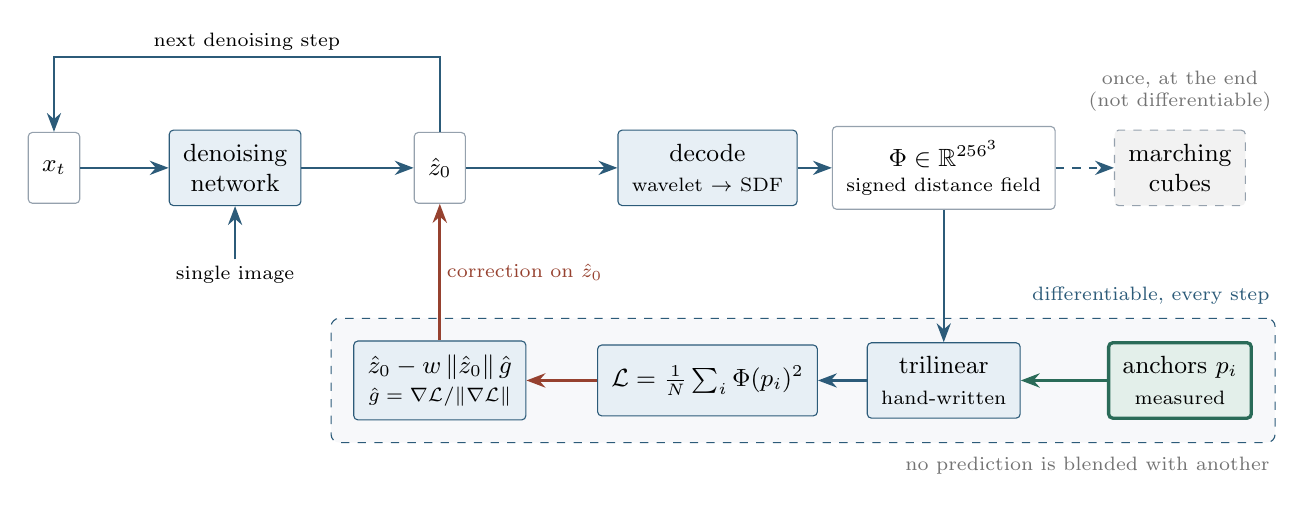
\begin{tikzpicture}[
  font=\small,
  >={Stealth[length=2.4mm]},
  box/.style    ={draw=lineC, fill=white, rounded corners=1.5pt, inner sep=5pt,
                  align=center, minimum height=9mm},
  op/.style     ={box, fill=accentL, draw=accent},
  data/.style   ={box, fill=white, draw=lineC},
  meas/.style   ={box, fill=goodL, draw=good, very thick},
  export/.style ={box, fill=black!5, draw=lineC, dashed},
  flow/.style   ={->, draw=accent, thick},
  back/.style   ={->, draw=bad, very thick},
  side/.style   ={->, draw=good, very thick},
  lbl/.style    ={font=\scriptsize, inner sep=2pt},
]

% ---- geometry --------------------------------------------------------------
\def\rowA{0}        % sampler row
\def\rowB{-2.7}     % geometric-residual row
\def\cA{0}   \def\cB{2.3}  \def\cC{4.9}
\def\cD{8.3} \def\cE{11.3} \def\cF{14.3}

% ---- top row: the sampler --------------------------------------------------
\node[data] (xt)   at (\cA,\rowA) {$x_t$};
\node[op]   (unet) at (\cB,\rowA) {\lblUnet};
\node[data] (z)    at (\cC,\rowA) {$\hat{z}_0$};
\node[op]   (dec)  at (\cD,\rowA) {\lblDec};
\node[data] (phi)  at (\cE,\rowA) {$\Phi \in \mathbb{R}^{256^3}$\\[-2pt]
                                   {\scriptsize\lblField}};

\draw[flow] (xt)   -- (unet);
\draw[flow] (unet) -- (z);
\draw[flow] (z)    -- (dec);
\draw[flow] (dec)  -- (phi);

% conditioning image enters the network from below, clear of the loop arrow
\node[lbl, align=center] (cond) at (\cB,-1.35) {\lblCond};
\draw[flow] (cond) -- (unet);

% ---- bottom row: the geometric residual ------------------------------------
\node[meas] (pts)  at (\cF,\rowB) {\lblContacts};
\node[op]   (int)  at (\cE,\rowB) {\lblInterp};
\node[op]   (loss) at (\cD,\rowB) {$\mathcal{L}=\frac{1}{N}\sum_i \Phi(p_i)^2$};
\node[op]   (grad) at (\cC,\rowB) {$\hat{z}_0 - w\,\lVert\hat{z}_0\rVert\,\hat{g}$\\[-1pt]
                                   {\scriptsize $\hat{g}=\nabla\mathcal{L}/\lVert\nabla\mathcal{L}\rVert$}};

\draw[side] (pts)  -- (int);
\draw[flow] (phi)  -- (int);          % vertical: columns are aligned
\draw[flow] (int)  -- (loss);
\draw[back] (loss) -- (grad);

% the correction returns to zhat_0 -- the whole point of the figure
\draw[back] (grad) -- (z)
  node[lbl, midway, right, text=bad, align=left] {\lblGrad};

% ---- the loop --------------------------------------------------------------
\draw[flow] (z.north) -- ++(0,0.95) -| (xt.north)
  node[lbl, pos=0.25, above] {\lblLoop};

% ---- outside the loop: mesh export -----------------------------------------
\node[export] (mc) at (\cF,\rowA) {\lblMc};
\draw[flow, dashed] (phi) -- (mc);
\node[lbl, above=1.5mm of mc, text=black!55, align=center] {\lblNote};

% ---- framing ---------------------------------------------------------------
\begin{scope}[on background layer]
  \node[fit=(grad)(loss)(int)(pts), draw=accent, dashed, rounded corners=3pt,
        inner sep=8pt, fill=accent!4] (boxA) {};
\end{scope}
\node[lbl, text=accent, anchor=south east, yshift=1mm] at (boxA.north east)
  {\lblBoxA};
\node[lbl, text=black!55, anchor=north east, yshift=-1mm] at (boxA.south east)
  {\lblBoxB};

\end{tikzpicture}
}
\caption{\textbf{Constraint anchoring, in place.} The correction acts on the predicted
$\hat{z}_0$ \emph{inside} the denoising loop, through a decode that is differentiable
end to end; the anchors are the only measured quantity in the diagram (green).
Marching cubes sits outside the loop because it is not differentiable --- and the
guidance never needs a mesh, only the field. Because no prediction is ever blended
with another, the destructive interference that condemns the composition-based
formulations of Sec.~\ref{sec:fusions} cannot occur.}
\label{fig:method}
\end{figure*}

The guidance never needs a mesh, only the field: marching cubes~\cite{marchingcubes}
is applied once at the end, to export the result. Crucially, \emph{no prediction is
ever blended with another}. The destructive interference that condemns the
composition-based formulations of Sec.~\ref{sec:fusions} cannot occur.

\textbf{Implementation.} $\mathcal{T}$ is written by hand as indexing and products
rather than with \texttt{grid\_sample}: the 3D backward kernel of the latter is
unimplemented on Apple Metal, and the CPU fallback would impose a 67\,MB round trip
per step. Measured cost: $3.44$\,s per guided step, $8.98$\,GB peak memory, $\approx
55$\,s per sample at 20 steps on an M2 Max --- no remote compute. The backbone's
weights are used unchanged, but its code is not the published one. Running it on Metal
required casting float64 tensors to float32 at several points and building the
sparse-convolution library natively; a backward pass through the model fits in memory
only with gradient checkpointing on the diffusion transformer (peak $21 \rightarrow
6.5$\,GB); and three pull requests of the public repository are merged in. The guidance
itself wraps the denoiser at sampling time and changes neither the sampler nor the
weights. The anchoring campaigns reported here all ran on that port, and none was
cross-checked against the reference CUDA implementation. The modified code is released
with the paper, with a notice listing these changes as the backbone's licence requires.

\textbf{Optional surface-normal term.} A contact from a hand carries an approximate
outward normal $n_i$. We impose only the \emph{direction} of the field gradient,
$\mathcal{L}_{\text{nrm}} = \frac{1}{N}\sum_i [\,1 - s\, g_i\!\cdot n_i / \lVert g_i
\rVert\,]$ with $g_i = \nabla_{\!p}\Phi|_{p_i}$ by central finite differences and $s =
+1$ the measured sign convention (exterior positive: interior median $-0.0998$,
exterior $+0.0999$, a TSDF truncated at $\pm 0.10$). The two losses have
incommensurable units; $\lambda$ is calibrated once at the first guided step so that
their gradient norms match, then frozen. Sec.~\ref{sec:res-anchor} shows the term does
not measurably help.

\textbf{Placing the anchors.} Without ground truth, the frame is estimated from two
criteria: \emph{silhouette consistency} (project the prediction and compare to the
conditioning image, which the model already received) and \emph{anchor residual}
(among silhouette-plausible poses, keep the one whose anchors lie closest to the
first-pass surface). Neither suffices alone. Registering anchors onto an unguided first
pass by ICP places them, against their exact position, at $0.66$--$0.76$ in median in
a frame where the object spans $[-1,1]$ --- \emph{on} the surface but in the
\emph{wrong place}, since ICP superimposes without respecting correspondences and
near-symmetries leave it that latitude. Silhouette plus residual brings the median gap
from $0.755$ to $0.501$, and to $0.111$ on objects without silhouette ambiguity.

\subsection{Anchoring by conditioning through a multi-view variant}
\label{sec:conditioning}

The four-view depth variant anchors the frame but demands four inputs, and four real
views leave no margin. Feeding one real view and three blank images fails: measured on
four objects and two seeds, $43.07$ \Fs{} against $95.40$ with four real views, and
worse than the dedicated single-view model on half the objects. \textbf{Blank views
are not neutral; they remove information.}

A depth map, however, is 3D geometry in the camera frame. It can be back-projected to
points and re-rendered from any other position of the canonical rig. The synthetic
view is geometrically correct where it has data and empty elsewhere --- far closer to
the training distribution than a black image. We therefore feed the model \emph{one
real depth view and three reprojected from it}, with their four camera indices. The
placement of anchors then becomes a fixed transform, calibrated once: measured on four
objects and two seeds, the output rotation stays between $118^\circ$ and $122^\circ$
about a constant axis.

The design intent was that the reprojection \emph{add no information} --- the same
single observation re-encoded --- so that reconstruction would stay at the single-view
level while the camera indices anchor the pose. Sec.~\ref{sec:res-conditioning} shows
that this intent was not met: the model treats the reprojected views as evidence, and
what it does with their holes depends on the object.

\subsection{Anchor model}
\label{sec:contactmodel}

Sampling anchors uniformly on the reference mesh is the heaviest objection against any
anchoring result, since the points then come from the answer. We replace it with a
palpation model imposing three physical constraints: straight-line reachability (rays
cast from outside, first hits only), restriction to the face hidden from the camera (a
camera placed in the wrong frame, so that $61\%$ of these anchors are hidden from the
one that rendered the image; see Limitations), and
rejection of points where a 6\,mm fingertip would not fit. Anchors are grouped into
\emph{sites} rather than scattered --- a hand touches in patches. This change alone
halves the ceiling of the method ($+14.37 \rightarrow +6.77$ on five objects): part
of the gain reported by intermediate campaigns came from uniform coverage, not from
the measurements.

For Sec.~\ref{sec:res-hand} we additionally use a \emph{grasp simulator} that places
one anchor per finger zone (thumb, index, middle, ring, little, palm) at fixed
anatomical angles around the object's principal axis, far closer to a real hand than
well-spread sites: minimum inter-anchor distance $0.058$--$0.344$ against
$0.446$--$1.281$ for our sites.

% ===========================================================================
\section{Experimental Setup}
% ===========================================================================

\textbf{Protocol.} 42 YCB objects~\cite{ycb}, 3 noise seeds each, giving 126
\emph{paired} comparisons: each anchored generation is compared to an unanchored one
with the \emph{same seed}. Because nothing is trained, every object is a test object.

\textbf{Metric.} F-Score@2\% after alignment to the reference, plus symmetric Chamfer
distance and connectivity.

\textbf{Significance.} We use a \textbf{sign test}, not a $t$-test: the gain
distribution is strongly skewed (median $+1.69$ for a mean of $+3.21$) and a few
objects dominate. A mean is fragile there; a count of signs is not. All $p$-values are
\textbf{two-sided}, and exact ties are discarded rather than counted as failures --- one
case out of 126 scores identically with and without anchoring, which is why the main
result is reported on 125.

\textbf{Oracle discipline.} Where stated, anchors are placed using the reference mesh, drawn with the palpation model of Sec.~\ref{sec:contactmodel}.
Such numbers are reported \emph{only} as upper bounds, never as system performance,
and always with an explicit statement of what was given for free.

% ===========================================================================
\section{Results}
% ===========================================================================

\subsection{Anchoring by constraint: what the frame costs}
\label{sec:res-constraint}

\begin{table}[t]
\centering
\caption{Constraint anchoring with tactile contacts, 42 YCB objects.}
\label{tab:main}
\begin{tabular}{lr}
\toprule
Unanchored baseline (image only) & 53.1 \Fs \\
\midrule
Mean gain, frame estimated & \gd{$+3.21$} \\
Median / std.\ dev. & $+1.69$ / $7.52$ \\
Positive cases & \gd{83 / 125} \\
Sign test (two-sided) & \gd{$p = 3.1\times10^{-4}$} \\
Objects with positive mean gain & 35 / 42 \\
\midrule
Mean gain, frame given (oracle) & $+7.82$ \\
\bottomrule
\end{tabular}
\end{table}

Table~\ref{tab:main} gives the constraint result. The effect is modest relative to its
spread --- it is the significance of the \emph{sign} that is solid, not the precision
of the magnitude. On five objects an earlier campaign measured $+1.79$ at $p = 0.035$;
at 42 objects the effect is stronger and two orders of magnitude more significant, so
it was not a single object carrying everything.

Comparing the realised gain to the oracle isolates the cost of estimating the frame:
$+3.21$ against $+7.82$ over 42 objects, and $+1.79$ against $+6.77$ under the
palpation model on five. \textbf{Frame estimation absorbs 59--74\% of what constraint
anchoring can deliver} --- an order of magnitude more than any other factor measured in
this paper.

\subsection{Anchoring by conditioning: the frame fixed, at a price}
\label{sec:res-conditioning}

\begin{table}[t]
\centering
\caption{The two anchoring routes, and their combination. Same 42 objects, same
126 seed-paired cases, same metric.}
\label{tab:routes}
\begin{tabular}{lrr}
\toprule
& \Fs & frame \\
\midrule
Image only (single-view backbone) & 53.1 & drawn with noise \\
\quad $+$ contacts as constraint & 56.3 & estimated, $\pm$ large \\
Depth reprojected to 4 views & \gd{64.3} & fixed, $\pm 2^\circ$ \\
\quad $+$ contacts as constraint & 64.7 & fixed \\
\midrule
Per-case oracle choice of route & 72.2 & --- \\
Four \emph{real} depth views (4 objects) & 98.6 & fixed \\
\bottomrule
\end{tabular}
\end{table}

Table~\ref{tab:routes} places the two routes side by side. Reprojecting a single
depth map into the four canonical views gains $+11.22$ over the single-view backbone in
paired mean --- more than three times what contacts deliver --- and fixes the frame.
But the gain is \textbf{bimodal}: 87 of 126 cases improve by $+26.1$ on average, and
39 cases lose $-22.1$. The losses are catastrophic on solids of revolution ---
baseball $95.5 \rightarrow 29.2$, soccer ball $93.9 \rightarrow 35.5$, master chef can
$91.0 \rightarrow 46.8$ --- where a single depth view leaves three canonical views
almost empty and the model fills them from its prior, badly. The design intent of
Sec.~\ref{sec:conditioning}, that reprojection add no information, was not met: the
model treats the reprojected views as evidence.

\textbf{No ground-truth-free selector we tested recovers the oracle.} A per-case
choice between the two routes would reach $72.2$. The obvious selector --- the fraction
of reprojected pixels that carry depth --- is \emph{anti}-correlated with the gain
($r = -0.40$): compact round objects fill many pixels and fail, thin flat ones fill few
and succeed. Coverage measures object shape, not reprojection quality, and no threshold
on it beats always choosing reprojection. Symmetry classification, the other candidate,
was already refuted as a predictor in Sec.~\ref{sec:res-anchor}. The $72.2$ exists but
is out of reach without knowing the answer.

\textbf{Stacking contacts on the anchored frame adds $+0.38$} (75/126 positive,
$p = 0.040$). Once the frame is fixed and the prior is strong, contacts have little
left to correct. The two routes are not complementary either: the correlation between
the reprojection gain and the contact gain is $+0.056$, and on the 39 cases where
reprojection fails, contacts recover $+1.7$ against a loss of $-22$. They fail on
different objects by accident, not by design.

\subsection{What an anchor set needs}
\label{sec:res-anchor}

\begin{figure*}[t]
\centering
\resizebox{\textwidth}{!}{%% ---------------------------------------------------------------------------
%% fig_results.tex -- results figure, shared geometry between icra_en/icra_fr.
%%
%% Requires the label macros \rlbl* to be defined by the calling document.
%%
%% Two panels, one claim each, and they answer each other:
%%   (a) seven controlled manipulations, all paired. Two families of standard
%%       error: 0.58 within a campaign (pooled over four objects; shared oracle frame, placement noise
%%       cancels) and 0.91 across campaigns (no shared unanchored pass). Colour
%%       encodes the two-sided sign test, which carries the conclusions. Three
%%       clear it, four do not -- and the three that do are all about WHERE the
%%       anchors are and how accurately they are placed, never how many there
%%       are or what the camera can see of them.
%%   (b) the visibility result on its own, because it is the one that runs
%%       against the premise of the work. Visibility is decided from the camera
%%       that rendered the images (tools/visibility_render_camera.py); the
%%       campaign's own fractions came from a camera placed in the wrong frame.
%%
%% All values are paired differences between two guided conditions on the same
%% object and the same seed; n = 15 each.
%% ---------------------------------------------------------------------------

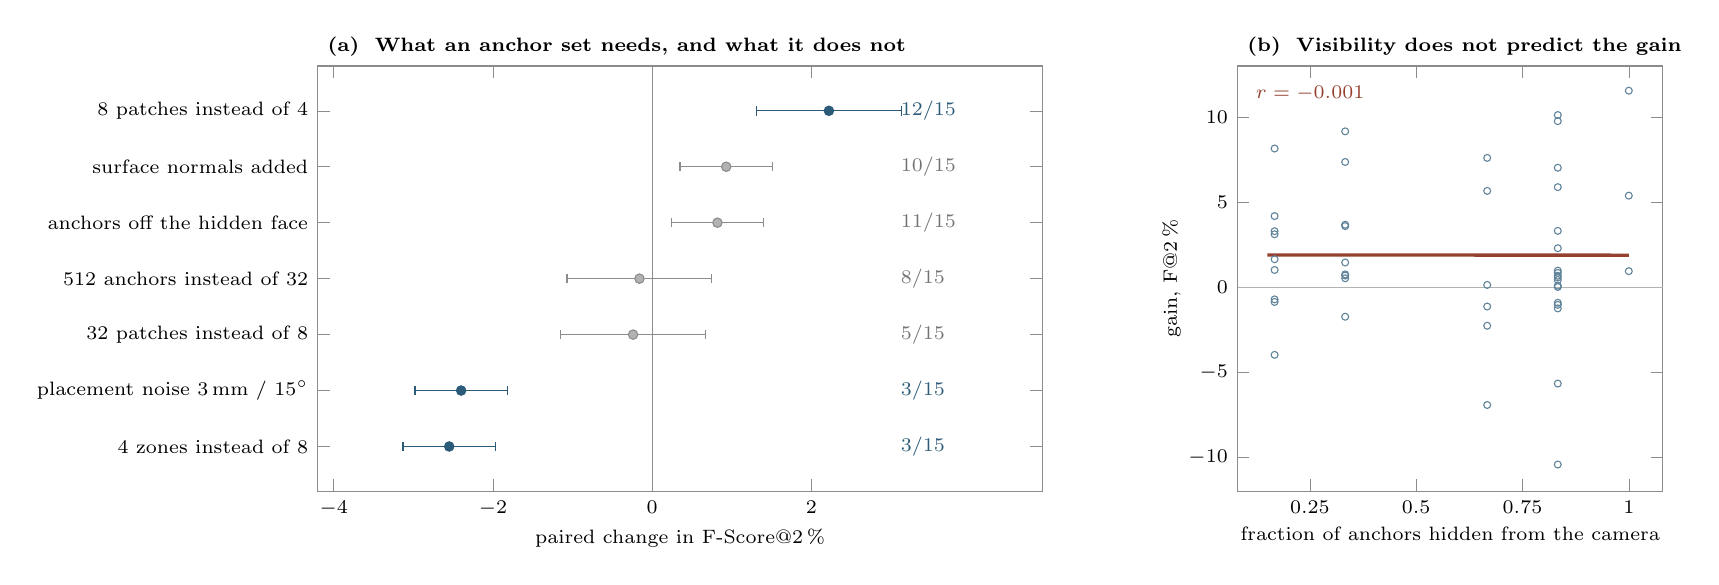
\begin{tikzpicture}

% ===== panel (a) : forest plot ==============================================
\begin{axis}[
  name=fa,
  width=9.2cm, height=5.4cm,
  scale only axis,
  xmin=-4.2, xmax=4.9,
  ymin=-0.8, ymax=6.8,
  ytick={0,1,2,3,4,5,6},
  yticklabels={\rlblZones,\rlblNoise,\rlblPatchHi,\rlblDens,\rlblVis,\rlblNorm,\rlblPatchLo},
  yticklabel style={font=\scriptsize, align=right},
  xtick={-4,-2,0,2},
  xticklabel style={font=\scriptsize},
  xlabel={\scriptsize \rlblXlab},
  xlabel style={yshift=2pt},
  axis line style={draw=black!45},
  tick style={draw=black!45},
  grid=none,
  clip=false,
]
  \draw[black!45] (axis cs:0,-0.8) -- (axis cs:0,6.8);

  % Barres d'erreur a une erreur type. ATTENTION, deux familles :
  %   0,58 quand les deux conditions partagent le repere oracle (meme campagne :
  %        le bruit de placement s'annule dans la difference appariee) ;
  %   0,91 quand elles viennent de campagnes distinctes, qui ne partagent aucune
  %        passe non guidee, et ou ce bruit ne s'annule pas.
  % La couleur encode le test des signes bilateral, pas ces erreurs types : c'est
  % lui qui porte les conclusions, parce qu'il ne demande aucune estimation de sigma.
  \addplot[only marks, mark=*, mark size=1.7pt, draw=accent, fill=accent,
           error bars/.cd, x dir=both, x explicit, error bar style={accent}]
    table[x=v, y=i, x error=e] {
      v      i   e
      -2.55  0   0.58
      -2.40  1   0.58
       2.22  6   0.91
    };
  \addplot[only marks, mark=*, mark size=1.7pt, draw=black!45, fill=black!30,
           error bars/.cd, x dir=both, x explicit, error bar style={black!45}]
    table[x=v, y=i, x error=e] {
      v      i   e
      -0.24  2   0.91
      -0.16  3   0.91
       0.82  4   0.58
       0.93  5   0.58
    };

  % le compte de signes, qui est l'evidence reelle
  \node[font=\scriptsize, text=accent,   anchor=west] at (axis cs:3.0,0) {3/15};
  \node[font=\scriptsize, text=accent,   anchor=west] at (axis cs:3.0,1) {3/15};
  \node[font=\scriptsize, text=black!55, anchor=west] at (axis cs:3.0,2) {5/15};
  \node[font=\scriptsize, text=black!55, anchor=west] at (axis cs:3.0,3) {8/15};
  \node[font=\scriptsize, text=black!55, anchor=west] at (axis cs:3.0,4) {11/15};
  \node[font=\scriptsize, text=black!55, anchor=west] at (axis cs:3.0,5) {10/15};
  \node[font=\scriptsize, text=accent,   anchor=west] at (axis cs:3.0,6) {12/15};

\end{axis}

\node[font=\scriptsize\bfseries, anchor=south west] at (fa.north west)
  {(a)\; \rlblPanelA};

% ===== panel (b) : occlusion vs gain ========================================
\begin{axis}[
  name=fb,
  at={(fa.right of east)}, anchor=left of west, xshift=14mm,
  width=5.4cm, height=5.4cm,
  scale only axis,
  xmin=0.08, xmax=1.08,
  ymin=-12, ymax=13,
  xtick={0.25,0.5,0.75,1},
  xticklabel style={font=\scriptsize},
  ytick={-10,-5,0,5,10},
  yticklabel style={font=\scriptsize},
  xlabel={\scriptsize \rlblXlabB},
  ylabel={\scriptsize \rlblYlabB},
  xlabel style={yshift=2pt}, ylabel style={yshift=-4pt},
  axis line style={draw=black!45},
  tick style={draw=black!45},
  clip=false,
]
  \draw[black!30] (axis cs:0.08,0) -- (axis cs:1.08,0);

  % the 45 cases, hidden fraction seen from the rendering camera
  \addplot[only marks, mark=o, mark size=1.25pt, draw=accent!75] coordinates {
    (0.333,1.45) (0.333,0.68) (0.333,0.75) (0.833,0.97) (0.833,0.84) (0.833,0.57)
    (0.167,1.64) (0.167,3.29) (0.167,1.01) (0.333,3.59) (0.333,-1.74) (0.333,3.67)
    (0.833,3.31) (0.833,2.29) (0.833,0.09) (0.167,4.18) (0.167,3.11) (0.167,8.15)
    (0.833,0.42) (0.833,-1.04) (0.833,0.67) (0.833,-10.43) (0.833,-1.25) (0.833,-0.92)
    (0.167,-3.98) (0.167,-0.72) (0.167,-0.87) (0.667,5.66) (0.667,-1.14) (0.667,-6.93)
    (0.833,7.02) (0.833,-5.67) (0.833,5.88) (0.667,7.60) (0.667,0.13) (0.667,-2.27)
    (0.833,10.12) (0.833,0.01) (0.833,9.76) (1.000,11.55) (1.000,0.94) (1.000,5.38)
    (0.333,9.16) (0.333,0.52) (0.333,7.36)
  };
  % least-squares fit: flat
  \addplot[draw=bad, very thick, domain=0.15:1.0, samples=2] {-0.013*x + 1.893};

  \node[font=\scriptsize, text=bad, anchor=north west] at (axis cs:0.10,12.4)
    {$r=-0.001$};
\end{axis}

\node[font=\scriptsize\bfseries, anchor=south west] at (fb.north west)
  {(b)\; \rlblPanelB};

\end{tikzpicture}
}
\caption{\textbf{Seven controlled manipulations of the anchor set.}
\textbf{(a)} Every estimate is a paired difference between two anchored conditions on
the same object and the same noise seed ($n=15$). Error bars are one standard error
--- $0.58$ when both conditions come from the same campaign and therefore share the
oracle frame, so that placement noise cancels in the difference (pooled over four
objects), and at least $0.91$ when they come from different campaigns, which share no
unanchored pass (measured on one object). Colour marks
significance under a two-sided sign test, whose counts are given at the right; we rely
on it rather than on the standard errors, because it needs no estimate of $\sigma$.
Only three comparisons clear it, and all three concern \emph{where} the anchors are
and \emph{how accurately} they are placed --- never how many there are, nor what the
camera can see of them. \textbf{(b)} The visibility result on its own, over the 45
cases of the grasp-strategy campaign, with visibility decided from the camera that
rendered the images. The least-squares fit is flat.}
\label{fig:results}
\end{figure*}

Fig.~\ref{fig:results}a sweeps seven properties of the anchor set under constraint
anchoring, on five objects, oracle placement. Three clear a two-sided sign test at
$p = 0.035$, and they share a theme.

\textbf{Spread matters.} At constant budget of 128 anchors distributed over $N$
sites, the gain is $-0.42$ at 4 sites, $+1.79$ at 8, $+2.03$ at 16 and $+1.55$ at 32:
a threshold between 4 and 8, then a plateau. Going from 8 patches to 4 costs $-2.55$
(12/15 negative).

\textbf{Placement accuracy matters.} Gaussian noise of $3$\,mm on position and
$15^\circ$ on normals, the order of what a finger's forward kinematics would deliver,
costs $-2.40$ (12/15 negative).

\textbf{Count does not.} From 32 to 512 anchors, the gain is $+0.23$, $+1.21$, $+0.07$:
flat over a $16\times$ range.

\textbf{Normals do not.} Adding them gives $+0.93$, which the sign test cannot separate
from zero ($10/15$, $p = 0.302$). The mean is carried by two outliers: dropping the
largest leaves $+0.43$, against a median of $+0.26$.

\textbf{Visibility does not --- and this is the result that overturns the premise.}
Using the grasp simulator, three strategies place the same six anchors with $87\%$,
$60\%$ and $30\%$ of them on the face hidden from the camera. Their gains are $+1.37$,
$+1.73$ and $+2.55$: the strategy that touches the hidden face \emph{least} gains
\emph{most}, although the sign test separates none of them ($11/15$, $p = 0.118$
between the last two). Case by case, over 45 cases, the correlation between hidden
fraction and gain is $r = -0.001$ (Fig.~\ref{fig:results}b): how many anchors the camera
cannot see says nothing about the gain. Sparse
anchors do not complete what vision misses. \textbf{They fix global position, scale
and orientation of a prior whose frame is loose, and for that it does not matter which
side they lie on.}

\subsection{Why fusion formulations fail}
\label{sec:fusions}

Five formulations require the measurements to produce a complete shape that is then
blended with the image's. The most instructive failure is weighted blending in
$\hat{z}_0$ space, which collapses from $44.9$ to $13.9$ \Fs{} at equal weight:
convex interpolation between two distinct modes of a distribution lands in a
low-density region --- the midpoint between two plausible shapes is not a plausible
shape. This holds for any naive blending of generative latents.

\begin{table}[t]
\centering
\caption{Six oriented contacts, with and without a generative prior. Poisson values are mean $\pm$ s.d.\ over five runs.}
\label{tab:poisson}
\begin{tabular}{lr}
\toprule
Poisson reconstruction~\cite{poisson}, 6 oriented contacts & $19.90 \pm 0.36$ \Fs \\
Poisson reconstruction, 18 contacts (3 grasps) & $20.44 \pm 0.18$ \\
\midrule
Generative prior, image only, no measurement & \gd{56.52} \\
\bottomrule
\end{tabular}
\end{table}

Table~\ref{tab:poisson} converts the shared cause into a measurement without any
diffusion model. Poisson reconstruction consumes exactly oriented points and yields a
watertight surface in 9 of 10 cases --- this is not gravel. It still reaches only
35\% of what the image alone already achieves. Sparse measurements are a poor
generator and a good anchor; the division of labour is not a design choice but what
the data imposes.

A \emph{learned} fusion module (a geometry encoder and cross-attention grafted onto
the frozen backbone, 50 epochs, 5--10\,M trainable parameters) measures $-4.20$ over
five objects with unpaired draws --- $0.9$ standard errors, indistinguishable from
zero. The comparison with constraint anchoring is not really about the two scores,
both poor. It is that the learned route \textbf{consumes the objects it would need in
order to judge itself}: 15 of 20 become training data, leaving five to conclude on,
with unpaired noise four times larger. In a small-data, noisy-metric regime a method
that needs no training buys \emph{statistical power}, and that decided this study.

\subsection{What survives at hardware cardinality}
\label{sec:res-hand}

\begin{table}[t]
\centering
\caption{Hardware-realistic cardinality, oracle placement. Paired differences below.}
\label{tab:hand}
\begin{tabular}{lrr}
\toprule
Condition & Mean gain & Sign test \\
\midrule
8 anchors, position only & $+3.25$ & $p=0.118$ \\
8 anchors $+$ normals & $+4.18$ & $p=0.118$ \\
8 anchors, noisy placement & $+1.78$ & $p=0.302$ \\
4 anchors only & $+0.70$ & $p=1.000$ \\
\midrule
\multicolumn{3}{l}{\emph{Paired differences (same object, same seed)}}\\
Normals vs.\ none & $+0.93$ & $p = 0.302$ \\
Placement noise 3\,mm / $15^\circ$ & \lo{$-2.40$} & \gd{$p = 0.035$} \\
4 zones instead of 8 & \lo{$-2.55$} & \gd{$p = 0.035$} \\
\bottomrule
\end{tabular}
\end{table}

A nine-zone dexterous hand excites only three to five zones in a real grasp. At one
anchor per zone (Table~\ref{tab:hand}), a $16\times$ reduction from the reference
campaign costs roughly half the ceiling ($+6.77 \rightarrow +3.25$), not all of it.
But the two effects that reach significance are precisely the two properties of a real
grasp: placement noise and reduced zone count. A real hand has both, and the joint
condition --- clustered simulator anchors, with normals, placement noise \emph{and}
estimated rather than oracle frame --- has not been measured. We record the prediction,
before measurement, that it will be null.

\subsection{Methodological results}
\label{sec:methodology}

\textbf{Run-to-run variance, and where it comes from.} Re-running an identical command
eight times --- same object, same seed, same anchors --- gives a standard deviation of
$0.49$ for the unanchored pass but $2.29$ for the anchored one, and $2.50$ for the
paired difference. The obvious reading, that guidance amplifies GPU non-determinism, is
\emph{wrong}, and we report it because we held it first. Those repetitions are not
identical: the oracle frame is re-estimated from each repetition's own unanchored pass,
so the anchor positions move. Freezing the frame separates the causes:

\begin{center}\small
\begin{tabular}{lcc}
\toprule
& re-estimated frame & frozen frame \\
\midrule
unanchored & 0.49 & 0.68 \\
anchored & \textbf{2.29} & \textbf{0.70} \\
paired difference & 2.50 & 1.29 \\
\bottomrule
\end{tabular}
\end{center}

With the placement frozen, the anchored pass is as reproducible as the unanchored one
($0.70$ against $0.68$): on this object, \textbf{91\% of the variance of an anchored
score comes from re-estimating where the anchors go}. Repeating the frozen-frame
measurement on three more objects gives anchored standard deviations of $1.74$, $0.40$
and $2.56$ against unanchored ones of $2.53$, $0.49$ and $2.19$ --- the anchored pass is
never noisier than the unanchored one, on any object. \textbf{Guidance amplifies
nothing.} What does vary is the object: the floor spans $0.40$ to $2.56$ across the
four, a factor of six. Much of it is the scorer, not the generator.
Re-scoring each saved mesh four times, without generating anything again, gives
standard deviations of $0.33$ to $2.23$ depending on the object. Pooled over the four,
the scorer alone has a standard deviation of $1.45$ where an anchored score has $1.60$,
and $1.03$ where an unanchored one has $1.72$: both the alignment and the F-Score sample
points at random, and the ICP occasionally settles in another basin, up to $8$ points
apart on the same mesh. With the frame frozen, generation itself adds little ($0.66$
at most, by difference). Our standard errors come from single scorings and therefore
include this noise; averaging several scorings per prediction would shrink them.
The frame problem of Sec.~\ref{sec:frame} therefore appears twice --- it consumes most
of the mean gain, and it dominates the variance.

This fixes the error model. Within one campaign the oracle frame is computed once per
(object, seed) and shared by every condition, so placement noise cancels in
condition-versus-condition differences; across campaigns it does not, since no two
share an unanchored pass. Pooled over the four objects, the frozen-frame $\sigma$ of an
anchored score is $1.60$, which puts the within-campaign standard error of a paired
difference at $0.58$ over 15 cases; the cross-campaign figure, $0.91$, was measured on
one object only and is a lower bound (Fig.~\ref{fig:results}a). Under these, the two
degradations sit at $4$ standard errors and more, and the two effects the sign test
rejects --- normals, visibility --- at $1.4$ to $1.6$. We nonetheless base every claim
on the sign test, which needs no estimate of $\sigma$ and gives the same verdict.

\textbf{F-Score is blind to fragmentation.} A scatter of disjoint shards near the true
surface scores well. On the banana: a 128-point cloud input yields 43 connected
components with 11\% of faces in the largest, and $47.83$ \Fs, against $34.48$ for an
image-only prediction that is a single closed surface. We report the number of
components and reject distance metrics below a threshold on the largest-component
ratio.

\textbf{F-Score is blind to mirror symmetry.} Building registration candidates from
SVD bases yields orthogonal but not necessarily right-handed frames: \textbf{5 of 15
registrations were reflections}. Fixed by forcing the determinant to $+1$.

\textbf{A badly initialised ICP fails silently.} Identity-initialised ICP leaves the
registration outside its basin of convergence, understating one object by up to $31$
points with no error signal. This changed the ranking between compared methods, and
was the source of the learned module's original ``$-8$ points'' verdict.

% ===========================================================================
\section{Limitations}
% ===========================================================================

\textbf{The missing control.} The visibility result says anchors on the visible face
work as well as anchors on the hidden face. The visible face is exactly what a depth
camera measures. The experiment that follows --- replacing tactile contacts with a
handful of depth points from the visible face, as constraints in
Eq.~\eqref{eq:loss} --- has not been run. If it gives the same $+3$, then the constraint
route needs no touch at all; if it gives less, contacts carry something specific.
Either answer is publishable, and we do not have it.

\textbf{A camera placed in the wrong frame.} Blender's OBJ importer turns each Y-up
mesh into its Z-up world, $(x, y, z) \mapsto (x, -z, y)$, before the camera at
$(2.2, -2.2, 1.8)$ renders it. Every occlusion computation placed that camera in the
mesh's own frame instead, $68^\circ$ from where it rendered: projected from there, the
reference silhouettes overlap the input images at $0.51$ on average over 42 objects,
against $0.95$ with the turn applied, and the visible/hidden label differs on $26\%$ of
the surface. We found it late. The hidden fractions of the grasp strategies and
Fig.~\ref{fig:results}b are recomputed from the rendering camera; from the misplaced
one the correlation read $-0.145$, and three cases seemed to leave no anchor on the
hidden face. Two artefacts keep the error. The palpation sites of
Sec.~\ref{sec:contactmodel} were restricted to the face hidden from the misplaced
camera: seen from the rendering camera, $61\%$ of their anchors are hidden ($15$ to
$90\%$ depending on the object), a mostly hidden set rather than a hidden-face set.
And the visible/occluded recall split, which no claim relies on, is unreliable. A
smaller defect adds to it: the renderer normalises objects to a maximum dimension of
$1.3$ where the occlusion code uses $2.0$; with the camera corrected, it changes the
label of $3$ of the $45$ grasp cases.

Images are synthetic Blender renders under a single camera and lighting condition.
Anchors are sampled on the reference mesh --- filtered for reachability, occlusion and
fingertip clearance, but noiseless and never false, except where noise is added
deliberately. No real object, sensor or robot is involved, although the robotic bench
that motivated this work exists and is operational. A single backbone family and a
single guidance weight were used; three seeds per object is few; secondary experiments
use five objects and one of them, the power drill, carries a large share of several
totals. Formulations 3, 4 and 7 of the fusion taxonomy are \emph{moot} in this data
regime rather than invalidated --- early-fusion retraining, the only route the
backbone's authors validate, was out of budget.

% ===========================================================================
\section{Conclusion}
% ===========================================================================

A single-view 3D generative prior can be anchored by sparse metric measurements, and
what limits the anchoring is not the measurements. Their number does not matter over a
$16\times$ range; their normals do not measurably help; whether they lie on the face
the camera cannot see does not matter either. What matters is whether they can be
placed in the frame the generator produces in --- and that frame is drawn with the
noise, so no estimator can learn it. Estimating it anyway costs 59--74\% of the
achievable gain, and it is what varies between runs: with the frame frozen, anchoring adds no variance on any of four objects.

Fixing the frame by conditioning is possible, and worth three times more than
constraint anchoring on average, but it is not free: the model treats the reprojected
evidence as real, and on a third of the objects the price is catastrophic, with no
selector in sight that does not already know the answer. Stacking constraints on the
fixed frame adds almost nothing.

The mechanism consistent with all of this is not that measurements complete what
vision misses. It is that \emph{a few true anchors regularise the output of a
generative prior} --- position, scale, orientation --- and that the prior's own frame
is what stands in the way. That is a more modest claim than the one this work set out
to make, and a more general one: it applies to touch, to depth, and to any sparse
metric signal a robot can bring.

\balance
\begin{thebibliography}{99}

%% Checked online on 2026-09-01: wala, ycb, smith2020, smith2021, suresh2022 and
%% dust3r were verified against arXiv / the publisher listing. The remaining entries
%% (dhariwal, cfg, zero123, poisson, marchingcubes, sdedit) are standard references
%% reproduced from memory -- re-check page numbers before submission.

\bibitem{wala}
A.~Sanghi, A.~Khani, P.~Reddy, A.~Rampini, D.~Cheung, K.~R.~Malekshan, K.~Madan, and
H.~Shayani, ``Wavelet Latent Diffusion (WaLa): Billion-parameter 3D generative model
with compact wavelet encodings,'' \emph{arXiv:2411.08017}, 2024.

\bibitem{dhariwal}
P.~Dhariwal and A.~Nichol, ``Diffusion models beat GANs on image synthesis,'' in
\emph{Adv.\ Neural Inf.\ Process.\ Syst. (NeurIPS)}, 2021.

\bibitem{cfg}
J.~Ho and T.~Salimans, ``Classifier-free diffusion guidance,'' in \emph{NeurIPS
Workshop on Deep Generative Models}, 2021.

\bibitem{zero123}
R.~Liu, R.~Wu, B.~Van~Hoorick, P.~Tokmakov, S.~Zakharov, and C.~Vondrick,
``Zero-1-to-3: Zero-shot one image to 3D object,'' in \emph{Proc.\ IEEE/CVF Int.\
Conf.\ Comput.\ Vis.\ (ICCV)}, 2023.

\bibitem{dust3r}
S.~Wang, V.~Leroy, Y.~Cabon, B.~Chidlovskii, and J.~Revaud, ``DUSt3R: Geometric 3D
vision made easy,'' in \emph{Proc.\ IEEE/CVF Conf.\ Comput.\ Vis.\ Pattern Recognit.\
(CVPR)}, 2024.

\bibitem{ycb}
B.~Calli, A.~Singh, A.~Walsman, S.~Srinivasa, P.~Abbeel, and A.~M.~Dollar, ``The YCB
object and model set: Towards common benchmarks for manipulation research,'' in
\emph{Proc.\ Int.\ Conf.\ Adv.\ Robot.\ (ICAR)}, 2015, pp.~510--517.

\bibitem{smith2020}
E.~J.~Smith, R.~Calandra, A.~Romero, G.~Gkioxari, D.~Meger, J.~Malik, and
M.~Drozdzal, ``3D shape reconstruction from vision and touch,'' in \emph{Adv.\ Neural
Inf.\ Process.\ Syst. (NeurIPS)}, vol.~33, 2020.

\bibitem{smith2021}
E.~J.~Smith, D.~Meger, L.~Pineda, R.~Calandra, J.~Malik, A.~Romero, and M.~Drozdzal,
``Active 3D shape reconstruction from vision and touch,'' in \emph{Adv.\ Neural Inf.\
Process.\ Syst. (NeurIPS)}, 2021.

\bibitem{suresh2022}
S.~Suresh, Z.~Si, J.~G.~Mangelson, W.~Yuan, and M.~Kaess, ``ShapeMap 3-D: Efficient
shape mapping through dense touch and vision,'' in \emph{Proc.\ IEEE Int.\ Conf.\
Robot.\ Autom.\ (ICRA)}, 2022, pp.~7073--7080.

\bibitem{poisson}
M.~Kazhdan and H.~Hoppe, ``Screened Poisson surface reconstruction,'' \emph{ACM Trans.\
Graph.}, vol.~32, no.~3, 2013.

\bibitem{marchingcubes}
W.~E.~Lorensen and H.~E.~Cline, ``Marching cubes: A high resolution 3D surface
construction algorithm,'' in \emph{Proc.\ SIGGRAPH}, 1987.

\bibitem{sdedit}
C.~Meng, Y.~He, Y.~Song, J.~Song, J.~Wu, J.-Y.~Zhu, and S.~Ermon, ``SDEdit: Guided
image synthesis and editing with stochastic differential equations,'' in \emph{Proc.\
Int.\ Conf.\ Learn.\ Represent.\ (ICLR)}, 2022.

\end{thebibliography}

\end{document}
